\documentclass{article}

\usepackage{amsmath}
\usepackage{amsfonts} % For math fonts.
\usepackage{amssymb} % For other math symbols not covered by amsmath.
\usepackage[pdftex]{graphicx} % For pictures, use \includegraphics[scale=decimal]{pic.png}; must be a .png file type.
\usepackage{multicol}
\usepackage{textcomp}
\usepackage[colorlinks = true, urlcolor = blue]{hyperref}
\usepackage{enumitem}
\usepackage{graphbox} 
\usepackage{subfig}
\usepackage{multicol}
\usepackage{nopageno}


\usepackage{tikz}
\usetikzlibrary{positioning, calc}
\usetikzlibrary{shapes.geometric,angles,quotes}
\usepackage{tikz-3dplot}


%page formatting
\usepackage{fullpage}
\setlength{\parindent}{0pt}


\newcommand{\tab}{\hspace*{0.25in}}
\newcommand{\csq}[1]{\reflectbox{''}#1''}  %This produces CS style quotes.
\newcommand{\csqt}[1]{\text{\reflectbox{''}#1''}}  %This produces CS style quotes as text.


\usepackage{listings}
\lstset
{ %Formatting for code in appendix
    language=Python,
    basicstyle=\footnotesize,
    numbers=left,
    stepnumber=1,
    showstringspaces=false,
    tabsize=2,
    breaklines=true,
    breakatwhitespace=false,
}


\begin{document}



%split_point

%\end{document}
Matt Priem \hfill fctns and strings quiz\\
section 1\\
\begin{enumerate}
	\item 
		(Game: heads or tails)  Write a \textbf{function} that lets the user guess whether the flip of a coin 
		results in heads or tails. The function randomly generates an integer 0 or 1, which 
		represents head or tail. The function returns if the guess is correct or incorrect. The argument for the function will be $guess$ 
		(the guess of the user, 0 for heads and 1 for tails).\\
		Hint: Use the following lines of code to create the function.
		\begin{verbatim}
		    from random import randint
		    value = randint(0,1) #picks a random integer. Either 0 or 1.
		\end{verbatim}
		\textbf{Examples:}
		\begin{itemize}
			\item  toss\_coin(0) $\rightarrow$ \csq{Correct!} (if the random value is 0) or \csq{Incorrect!} (if the random value is 1), 
			\item  toss\_coin(1) $\rightarrow$ \csq{Correct!} (if the random value is 1) or \csq{Incorrect!} (if the random value is 0) 
		\end{itemize}

	\item 
		%https://edabit.com/challenge/sfqudQHQ3HPpd7dZb
		Write a \textbf{function} to create a game of Rock, Paper, Scissors. The function will return the winner of the game played by two players.
		The arguments to the function will be $player1$ (the first player's choice) and $player2$ (the second player's choice).\\
		Print the winner according to the following rules. 
		\begin{itemize}
			\item Rock beats Scissors
			\item Scissors beats Paper
			\item Paper beats Rock
		\end{itemize}		
		\textbf{Examples:}		
		\begin{itemize}
			\item  find\_winner(\csq{Rock}, \csq{Paper}) $\rightarrow$ \csq{Player 2 wins!}, 
			\item  find\_winner(\csq{Scissors}, \csq{Paper}) $\rightarrow$ \csq{Player 1 wins!}, 
			\item  find\_winner(\csq{Rock}, \csq{Rock}) $\rightarrow$ \csq{It's a tie!}
		\end{itemize}


	\item 
		%https://edabit.com/challenge/Mv5qSgZKTLrLt9zzW
		A fruit juice company tags their fruit juices by concatenating the first 
		\textbf{three letters} of the words in a flavor's name, with its capacity. 
		Create a function that creates product IDs for different fruit juices.
		Notice that the first input is a string and the second is an integer.
		
	\textbf{Examples:}
		\begin{itemize}
			\item get\_drink\_ID(\csq{apple}, 500) $\rightarrow$ \csq{app500}
			\item get\_drink\_ID(\csq{pineapple}, 45) $\rightarrow$ \csq{pin45}
			\item get\_drink\_ID(\csq{watermelon}, 750) $\rightarrow$ \csq{wat750}
		\end{itemize}
















\end{enumerate}
\pagebreak
Bart Simpson \hfill fctns and strings quiz\\
section 1\\
\begin{enumerate}
	\item 
		You are counting points for a tennis match. Write a \textbf{function} that 
		calculates the total points for a player and returns the value. The arguments for the function will be 
		$aces$ (each ace is worth 2 points) and $winning\_shots$ (each winning shot is worth 1 point).\\

	\textbf{Examples:}
	\begin{itemize}
		\item total\_score(1, 1) $\rightarrow$ 3, 
		\item total\_score(2, 3) $\rightarrow$ 7, 
		\item total\_score(5, 3) $\rightarrow$ 13
	\end{itemize}

	%new
	\item 
		Write a \textbf{function} that loops through and returns the sum of all odd numbers 
		between two integers (inclusive). The arguments to the function will be $smaller\_num$ 
		and $larger\_num$.

		\textbf{Examples:}		
		\begin{itemize}
			\item  odd\_sum(0, 7) $\rightarrow$ 16 (since 1+3+5+7 = 16)
			\item odd\_sum(1,10) $\rightarrow$ 25 (since 1+3+5+7+9 = 25)
			\item  odd\_sum(50, 517) $\rightarrow$ 66456 
		\end{itemize}


	\item
		Write a function called \textit{flip\_flop} that takes a string as an argument 
		and returns  a new word made up of the second half of the word first combined 
		with the first half of the word second.

		\textbf{Examples:}
		\begin{itemize}
			\item \textit{flip\_flop}(\csq{abcd}) $\rightarrow$ \csq{cdab} 
				(that is, \csq{cd} then \csq{ab} \dots even length)
			\item \textit{flip\_flop}(\csq{grapes}) $\rightarrow$ \csq{pesgra} 
				(that is, \csq{pes} then \csq{gra} \dots even length)
			\item \textit{flip\_flop}(\csq{abcde})$\rightarrow$ \csq{decab}
				(that is, \csq{de} then \csq{c} then \csq{ab} \dots odd length)
			\item \textit{flip\_flop}(\csq{cranberries})$\rightarrow$ \csq{rriesecranb}
				(that is, \csq{rries} then \csq{e} then \csq{cranb} \dots odd length)

		\end{itemize}











\end{enumerate}
\pagebreak
Lone Star \hfill fctns and strings quiz\\
section 2\\
\begin{enumerate}
	\item 
		A toy store owner wants to know the total number of batteries needed for all the electronic toys in the store. 
		The store sells three types of toys:
		\begin{itemize}
			\item Electronic dolls, which require \textbf{2} batteries
			\item Remote-controlled cars, which require \textbf{4} batteries
			\item Robot dogs, which require \textbf{6} batteries
		\end{itemize}


		Write a \textbf{function} that counts the total number of batteries needed for the toy store and returns the value. 
		The arguments for the function will be $e\_dolls$ (number of electronic dolls toy store has), $rc\_cars$ 
		(number of remote-controlled cars toy store has), and $robo\_dogs$ (number of robot dogs toy store has).\\

	\textbf{Examples:}
	\begin{itemize}
		\item  battery\_counter(4, 3, 2) $\rightarrow$ 32, 
		\item  battery\_counter(1, 1, 1) $\rightarrow$ 12, 
		\item  battery\_counter(0, 10, 0) $\rightarrow$ 40 
	\end{itemize}


	\item 
		%https://edabit.com/challenge/xR248CxGSsSrNK5Za
		You are the newest rug fashion designer on the scene, but you're running out of ideas. 
		Write a \textbf{function} that will help you design rugs.  The function will return a 
		formatted string that will resemble a designed rug. The first parameter must be $width$ 
		(how wide the rug will be), the second must be $length$ (how long the rug will be), 
		and the third must be $pattern$ (the character pattern used in the rug design).

		\textbf{Examples:} \\
			design\_run(3,5,\$) $\rightarrow$	\begin{tabular}{l}
			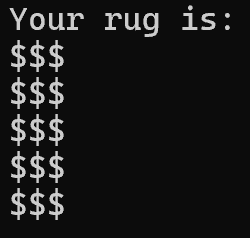
\includegraphics[height=1in]{./imgs/rug1_alt.PNG} \hspace{0.5in} \end{tabular}
			design\_run(16,5,\@) $\rightarrow$ \begin{tabular}{l}
			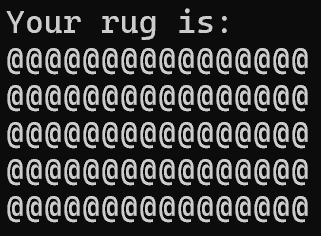
\includegraphics[height=1in]{./imgs/rug2_alt.PNG} \end{tabular}


	%new
	\item 
		Professor Dumbledore seeks to decipher powerful encoded spells in the Hogwarts Library, 
		their secrets revealed by the first letter of each word. Create a function called 
		$first\_letters$ that takes the variable $sentence$ (a string) and returns
		a string made up of the first letters of each word in the sentence. 

		\textbf{Examples:}
		\begin{itemize}
			\item first\_letters(\csq{wingardium leviosa makes objects float}) 
				$\rightarrow$ \csq{wlmof}
			\item first\_letters(\csq{expecto patronum repels dementors}) $\rightarrow$ \csq{eprd}
			\item first\_letters(\csq{the magic is within you}) $\rightarrow$ \csq{tmiy}
		\end{itemize}

\end{enumerate}
\pagebreak
Dot Matrix \hfill fctns and strings quiz\\
section 3\\
\begin{enumerate}
	%new
	\item 
		Write a \textbf{function} that loops through and returns the sum of all odd numbers 
		between two integers (inclusive). The arguments to the function will be $smaller\_num$ 
		and $larger\_num$.

		\textbf{Examples:}		
		\begin{itemize}
			\item  odd\_sum(0, 7) $\rightarrow$ 16 (since 1+3+5+7 = 16)
			\item odd\_sum(1,10) $\rightarrow$ 25 (since 1+3+5+7+9 = 25)
			\item  odd\_sum(50, 517) $\rightarrow$ 66456 
		\end{itemize}


	\item 
		%https://edabit.com/challenge/b8wRDMWgMZTN2nmfx
		Write a \textbf{function} that returns the number of copies of the same number. The arguments for the function will be $num\_1$ (first number), 					$num\_2$ (second number), and $num\_3$ (third number).\\

		\textbf{Examples:}		
		\begin{itemize}
			\item  count\_duplicates(2, 3, 2) $\rightarrow$ \csq{You entered the same number 2 times}, 
			\item  count\_duplicates(4, 4, 4) $\rightarrow$ \csq{You entered the same number 3 times}, 
			\item  count\_duplicates(1, 2, 3) $\rightarrow$ \csq{Each number is unique} 
		\end{itemize}


	\item 
		The \textbf{normal human body temperature} is 98.6F in Fahrenheit and 37C in Celsuis. 
		Create a function that determines if the \textit{temp} is considered a fever(anove normal 
		body temperature) or not.
		\textit{temp} will be measured in Fahrenheit and Celsuis.\\
		Notice: The F or C will always be the last character in the string.

	\textbf{Examples:}
	\begin{itemize}
		\item is\_fever(\csq{99F}) $\rightarrow$ True, 
		\item is\_fever(\csq{37C}) $\rightarrow$ False, 
		\item is\_fever(\csq{98F}) $\rightarrow$ False, 
	\end{itemize}

\end{enumerate}
\pagebreak
Alfred Yankovic \hfill fctns and strings quiz\\
section 2\\
\begin{enumerate}
	%new
	\item 
		In an Ancient Kingdom, the currency consists of bronze coins, silver coins, and gold coins.  There are 20 bronze coins in 
		one silver coin and 15 silver coins in one gold coin.  Write a \textbf{function} that will return a converted amount of 
		bronze coins into the fewest amount of coins possible.  Only return a string with the non-zero values, 
		meaning don't return something similar to ``0 silver coins''.  The argument for the function will be 
		$bronze\_coins$ (how many bronze coins to convert). 

		\textbf{Examples:}
		\begin{itemize}
			\item  convert\_bronze(32) $\rightarrow$ \csq{1 silver 12 bronze}, 
			\item  convert\_bronze(544) $\rightarrow$ \csq{1 gold 4 silver 4 bronze}, 
			\item  convert\_bronze(903) $\rightarrow$ \csq{3 gold 3 bronze}\\
				Note: Do \textbf{not} output 3 gold 0 silver 3 bronze.
		\end{itemize}

	\item 
		The table below show what your resting heart rate should be based on age and athleticism. 
		Write a \textbf{function} that returns what the resting heart rate of the user should be. 
		The arguments for the function will be $age$ (how old the user is) and $athl\_goal$ (athletic goal of user).
	\begin{center}
		\begin{minipage}{.45\textwidth}
			\begin{tabular}{c|cc}
				& \multicolumn{2}{c}{Athleticism}\\
				Age & Above Average & Below Average \\ \hline
				20 -- 39 & 47 -- 72 & 73 -- 93\\
				40 -- 59 & 46 -- 71 & 72 -- 94\\
				60 -- 79 & 45 -- 70 & 71 -- 97 \\
			\end{tabular}
		\end{minipage}
	\end{center}

	\textbf{Examples:}
	\begin{itemize}
		\item  resting\_rate(45, \csq{Below Average}) $\rightarrow$ \csq{72-94}, 
		\item  resting\_rate(79, \csq{Above Average}) $\rightarrow$ \csq{45-70}, 
		\item  resting\_rate(20, \csq{Below Average}) $\rightarrow$ \csq{73-93} 
	\end{itemize}


	\item 
		%https://edabit.com/challenge/Mv5qSgZKTLrLt9zzW
		A fruit juice company tags their fruit juices by concatenating the first 
		\textbf{three letters} of the words in a flavor's name, with its capacity. 
		Create a function that creates product IDs for different fruit juices.
		Notice that the first input is a string and the second is an integer.
		
	\textbf{Examples:}
		\begin{itemize}
			\item get\_drink\_ID(\csq{apple}, 500) $\rightarrow$ \csq{app500}
			\item get\_drink\_ID(\csq{pineapple}, 45) $\rightarrow$ \csq{pin45}
			\item get\_drink\_ID(\csq{watermelon}, 750) $\rightarrow$ \csq{wat750}
		\end{itemize}
















\end{enumerate}
\pagebreak
\end{document}